\section{The IDE}

The \tuprolog\ system comes with a simple application providing an user friendly integrated development environment to interact with a \tuprolog\ engine, manipulate its knowledge base, make queries and explore solutions.
%
In addition, means to dynamically manage the loading and unloading of \tuprolog\ libraries are provided.
%
After a proper installation of the \tuprolog\ distribution, the application is spawned by launching the executable class \classname{alice.tuprologx.ide.GUILauncher}.
%
The console user interface version, providing a command-line shell, can be accessed by launching the executable class \classname{alice.tuprologx.ide.CUIConsole}.

\begin{figure}
\centering
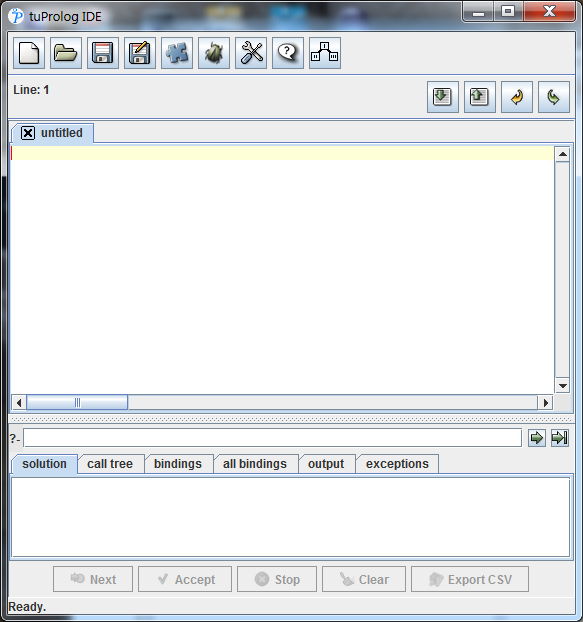
\includegraphics[scale=0.60]{images/tuPrologIDE}
\caption{\tuprolog\ IDE.}
\label{tuprolog-ide}
\end{figure}

The main window of the \tuprolog\ IDE is shown in \figref{tuprolog-ide}.
%
It is divided in two sections:
%
\begin{itemize}
\item an editing area on the middle, providing means to edit the engine's current theory;
\item a console on the bottom, providing means to ask queries and display their solutions.
\end{itemize}
%
In the main window there also are:
%
a toolbar at the top, providing facilities to manage theories, such as load, save as well as create a new theory, to load and unload libraries into and from the \tuprolog\ engine, and to view in a separate window the debug informations activated by means of the \predicate{spy/0} predicate;
%
and a status bar at the very bottom, providing status informations for the IDE and the engine.

\subsection{Editing the theory}

The editing area allows multiple theories to be created and modified at the same time, by allocating a tab with a new text area for each theory.
%
The text area provides syntax highlighting for comments, string and list literals, and predefined predicates.
%
Undo and Redo actions are supported through the usual \keycap{Ctrl}+\keycap{Z} and \keycap{Ctrl}+\keycap{Shift}+\keycap{Z} key bindings.

\begin{figure}
\centering
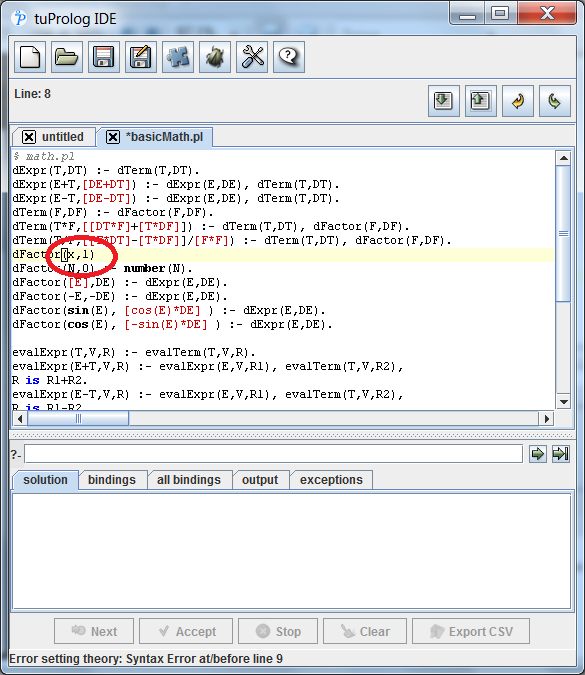
\includegraphics[scale=0.60]{images/syntaxErrorFound}
\caption{A syntax error is found when setting the content of the editor area as the new engine's theory.}
\label{syntax-error-found}
\end{figure}

\begin{figure}
\centering
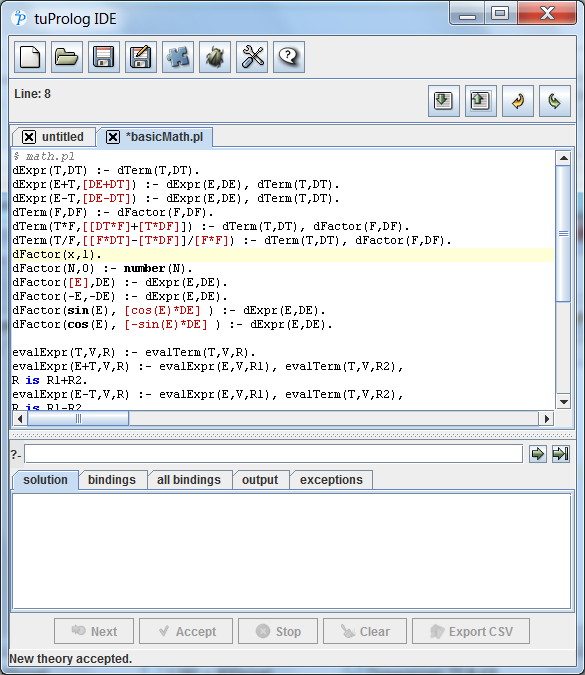
\includegraphics[scale=0.60]{images/setTheorySucceeded}
\caption{The syntax error is removed and the \guibutton{Set Theory} operation succeeds.}
\label{set-theory-succeeded}
\end{figure}

Above the editing tabs, a control area is found, where two buttons are provided to get the text of the engine's current theory into a new tab and to set the text contained in the editor of the selected tab as a new theory for the engine, and two buttons are provided for mouse-clicking support of Undo and Redo
actions.
%
An apposite action for retrieving the engine's current theory in an editor (shown in \figref{syntax-error-found}) is needed because whenever that theory gets modified by other means, such as calling the \texttt{consult/1} predicate, the changes are not automatically reflected in any text area.
%
On the left side of the control area, there also is an indicator of the line where the caret is currently positioned in the edit area.
%
Informations about the result of the action issued by the control area are provided in the status bar at the very bottom of the IDE's window:
%
for instance, when setting an invalid theory to the engine because of syntax errors, details about the error are provided.

\subsection{Solving goals}

The console at the bottom of the tuProlog IDE's window is subdivided in two logical panes:
%
\begin{itemize}
\item a query pane composed by a textfield where queries can be inserted, and two buttons to trigger the solving process.
%
The leftmost (\guibutton{Solve}) button asks the engine to find the first solution to the query, allowing the user to possibly navigate through further solutions;
%
the rightmost (\guibutton{Solve All}) button forces the engine to find all solutions to the given query.
%
Pressing the \keycap{Enter} key in the textfield has the same effect as pressing the \guibutton{Solve} button.
\item an answer pane, where answers and output informations are visualized.
%
Answers to Prolog queries are composed by both solutions, showed in a free form within a read-only text area, and bindings, displayed in tabular form.
%
The output tab provides a read-only view on the standard output where informations are possibly written by Prolog programs, by means of the I/O predicates supplied by the \classname{IOLibrary}.\footnote{The information written on standard output by methods invoked on Java objects from the \classname{JavaLibrary} -- for instance using the \varname{stdout} object -- are not displayed on this view.}
%
Control buttons are also provided to iterate through possibly multiple solutions, clear the bindings and output panes, and export tabular data in a convenient CSV format.
\end{itemize}
%
Goals are asked through the query input box, and answers (bindings and solutions) are provided in the related text area.
%
Query and answers are traced in a proper chronological history, that can be explored by means of \keycap{Up} and \keycap{Down} arrow keys from the query input textfield.
%
When open alternatives are found solving a goal, the \guibutton{Next} and \guibutton{Accept} buttons are enabled in the answer pane to interact with the engine, in order to let the user specify if the current solution is accepted or if other alternatives need to be explored.

Note that the theory contained in the currently selected edit pane does not have to be explicitly feeded to the Prolog engine before it could be possible to solve queries against that theory's knowledge base.
%
In fact, any time a goal is asked to be solved, the theory contained in the active edit area is automatically feeded to the engine if its knowledge base has been modified since the last solved goal.
%
(This obviously happens also on the first time a query is asked.)
%
However, whenever the engine's theory is modified by other means than the editor, it does need to be explicitly acquired and presented to the programmer in the text area.
%
In fact, if the theory in the engine is augmented by a call to the predicate \predicate{consult/1} issued from a query, for example, the contents of the newly consulted theory will not be automatically inserted in the editor:
%
when the programmer needs an up-to-date view of the knowledge base contained in the underlying \tuprolog\ engine, its display has to be explicitly triggered by means of the \guibutton{GetTheory} button, available
in the editing area.

An example of the user interaction involving multiple solutions is shown in the following sequence of figures:
%
in \figref{query-issued}, the user issued the query \userinput{test\_color(test, X).}, using the knowledge base written in the edit area (a solution to the Map Coloring problem,\footnote{The problem is to color a planar map so that no two adjoining regions have the same color. A famous conjecture was proved in 1976 showing that four colors are sufficient to color any planar map.} with a test map composed of six areas).
%
The first solution is displayed, and multiple open alternatives can be explored:
%
in \figref{next-solution-asked}, the user asked to get the next possible solution by pressing the \guibutton{Next} button, and another solution is provided;
%
finally, in \figref{accept-solution}, the user, after having explored the first two solutions, accepts the third one by pressing the \guibutton{Accept} button.
%
During the resolution of a goal, all the theory-related buttons are disabled, included the \guibutton{Library Manager} button, since each library can have its theory to be feeded into the engine.

\begin{figure}
\centering
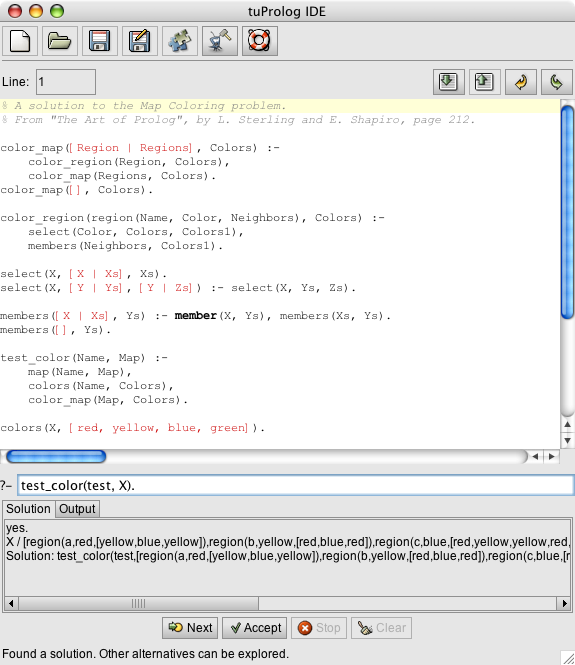
\includegraphics[scale=0.605]{images/queryIssued}
\caption{The user issued a query \userinput{test\_color(test, X).} and the first solution is displayed.}
\label{query-issued}
\end{figure}

\begin{figure}
\centering
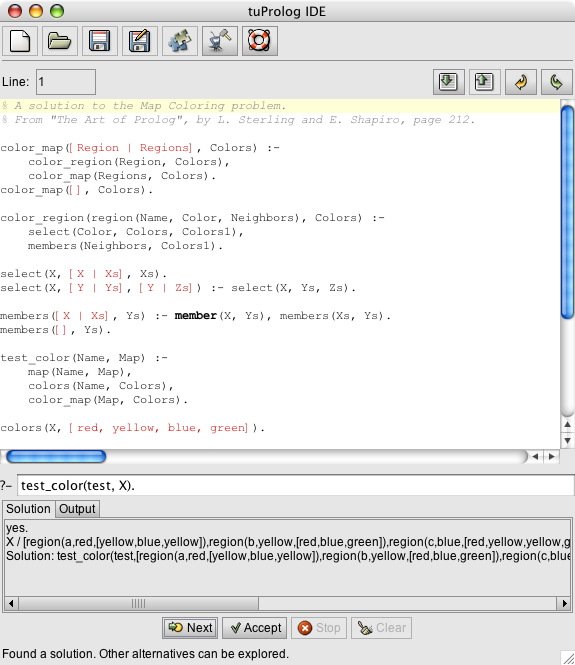
\includegraphics[scale=0.605]{images/nextSolutionAsked}
\caption{The user issued a \guibutton{Next} command and got another solution.}
\label{next-solution-asked}
\end{figure}

\begin{figure}
\centering
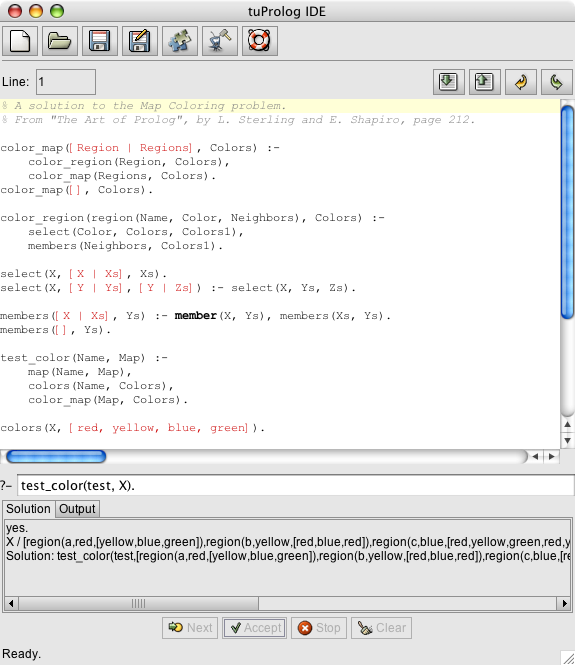
\includegraphics[scale=0.605]{images/acceptSolution}
\caption{The user accepted the third solution by pressing the \guibutton{Accept} button.}
\label{accept-solution}
\end{figure}

Near to the \guibutton{Next} and \guibutton{Accept} buttons, a \guibutton{Stop} button is found, providing the user with a means to halt the engine if a computation takes too long or a bug in the knowledge base feeded to the engine results in an infinite loop.

% Such a bug is contained in the following theory:
% \begin{verbatim}
% p(a).
% p(b) :- p(b).
% p(c).
% \end{verbatim}
% When solving a goal like \code{p(b)} or asking for the second solution to the query \code{p(X)}, the \tuprolog\ engine
% will be trapped in an infinite loop due to the particular recursive nature of the second clause in the feeded theory.
% By pressing the \guibutton{Stop} button, which is enabled only during computations, the user will be able to halt the
% engine and perform the necessary changes to the knowledge base before issuing another query, instead of being forced
% to close and reopen the IDE.

Finally, a \guibutton{Clear} button is provided, with the aim of allowing the user to clear the bindings and output panes when they get overfull with informations.
%
The button is enabled only when the proper tabs are selected.

\subsection{Debug Informations}

By pressing the \guibutton{View Debug Information} button, a new window is opened, providing a view on the warnings, produced by events such as the attempt at redefining a library predicate, and the spy information, concerning basic steps of the engine computation and state, possibly supplied by the engine during a goal demonstration:
%
Warnings are always active;
%
in order to activate the spy information notification, the \predicate{spy/0} built-in predicate (provided by \classname{BasicLibrary}) must be issued;
%
\predicate{nospy/0} can be used to stop this notification.
%
As an example, \figref{view-debug-information} shows the content of the spy information view after the
execution of a goal involving the activation of spy inspection.

It is worth noting that a computation may contain a huge number of traced steps.
%
For this reason, a toolbar at the top of the window allows to collapse and expand all nodes in the spy information pane, or to expand and collapse selected nodes only.
%
Finally, the content of the warnings and spy panes can be cleared using the \guibutton{Clear} button at the leftmost end of the toolbar.

\begin{figure}
\centering
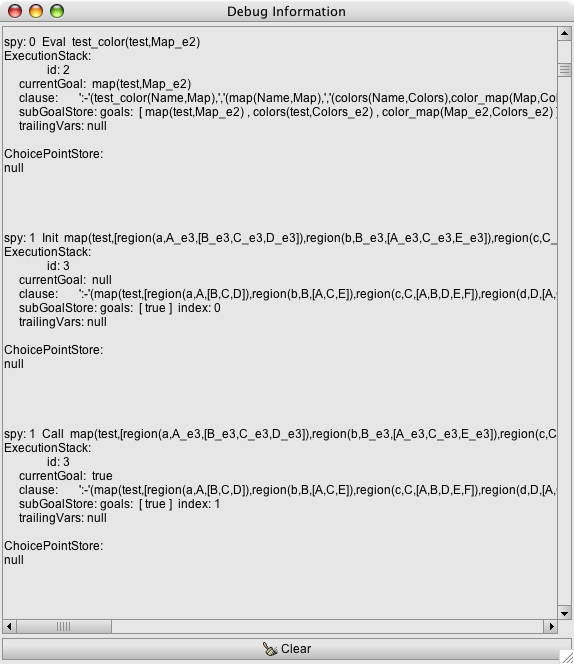
\includegraphics[scale=0.605]{images/viewDebugInformation}
\caption{Debug Information View after the execution of a goal.}
\label{view-debug-information}
\end{figure}

\subsection{Dynamic library management}


A \tuprolog\ engine can be extended by loading any number of libraries, each provinding a specific set of built-in
predicates and functors, and a related theory. The \tuprolog\ IDE allows a dynamic management of libraries through a
GUI dialog, which can be displayed by pressing the \guibutton{Open Library Manager} button in the toolbar. The Library
Manager dialog is shown in \figref{library-manager-dialog}.

\begin{figure}
\centering
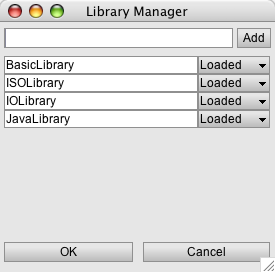
\includegraphics[scale=0.605]{images/libraryManagerDialog}
\caption{The Library Manager dialog.}
\label{library-manager-dialog}
\end{figure}

This dialog displays a list of the libraries currently loaded into the \tuprolog\ engine. For a new instance of the
engine, that list will typically contain the four standard libraries coming with the application core, that is
\classname{BasicLibrary}, \classname{IOLibrary}, \classname{ISOLibrary}, \classname{JavaLibrary}, along with their
current status. The user can add a library to the Library Manager simply by providing the fully qualified name of the
library's class in the textfield on the top of the dialog, then pressing the \guibutton{Add} button: the added library
will be displayed with an initial Unload status. The user can further select the status of each library in the list,
and commit changes to the \tuprolog\ engine by pressing the \guibutton{OK} button, or dismiss the dialog by pressing
the \guibutton{Cancel} button.

The library manager is also capable of updating itself accordingly to the events of libraries load and unload fired by
the \tuprolog\ engine.  Such events are triggered by the use of the \verb|load_library/1| and \verb|unload_library/1|
predicates or directives in query issued or theories feeded to the engine. So, if an user asks to solve the goal \verb|load_library('TestLibrary'), test(X).|,
for example, the manager would immediately reflect the change occurred in the engine's libraries pool, adding a new
entry if \verb|TestLibrary| had not been previously loaded or, if necessary, changing the library's entry status to
show the result of the loading action.

Both the action of adding a library to the manager and the action of loading a library into the engine can fail. If,
for example, the classname provided does not identify a \tuprolog\ library (i.e. it identifies a class not extending the
\classname{alice.tuprolog.Library} class) or the identified class does not exist, an appropriate message will appear
in the status bar at the bottom of the dialog. When adding or loading a library, please remember that every class
needed by that library must be in the classpath in order to have the library correctly added to the manager's list or
loaded into the engine. 